\subhead{Reading the selected bits}
A low Ising energy becomes a material recommendation only after the binary state has been decoded and compared across blocks. Figure~\ref{fig:decode} follows the Q3 winner. Holding Sn and Ti fixed, the three family scores are 3.2681 for O3, 8.2041 for FO2 and 12.3445 for NO2. The envelope stores the first value together with the O3 family and original row ID 8760.

\begin{figure}[htbp]
\centering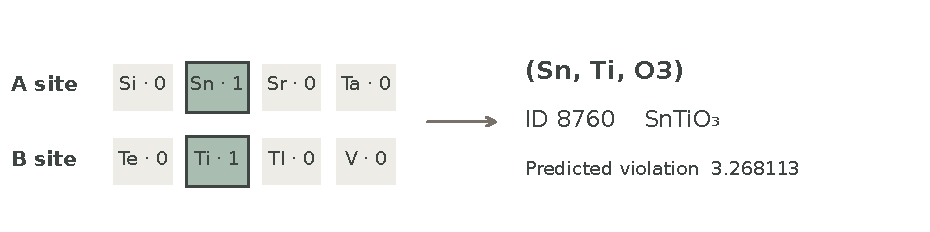
\includegraphics[width=\linewidth]{figures/qubo_decode.pdf}
\caption{Readout of the winning Q3 block. Each register contains exactly one active bit. Combining Sn and Ti with the stored minimizing family returns the full-pool material shown in Table~\ref{tab:answers}.}\label{fig:decode}
\end{figure}

The ordering $(\mathrm{Si,Sn,Sr,Ta})$ on A and $(\mathrm{Te,Ti,Tl,V})$ on B makes the second bit active in each register. If $\sigma_i$ is a returned spin and $\sigma_r$ the reference spin, the implemented readout is
\[
 z_i=\tfrac12(1+\sigma_i\sigma_r).
\]
Simultaneously reversing every spin leaves every product unchanged. The two gauge representations therefore identify the same pair and should be counted once. Fixing the reference to $+1$ gives binary vectors $(0,1,0,0)$ on both sides. The winning state's measured SDK energy is $-724$ and the decoded raw score is 3.268113. The block's lowest integer cost has one legal pair. Other blocks have different scale factors and omitted constants; their winners enter the final comparison through their raw scores.
